\graphicspath{{chapter3/figures/}}
\chapter{Explainable fully automated CT scoring of systemic sclerosis related interstitial lung disease by cascaded regression neural networks and its comparison with experts}
\label{chap:2}

% This is for title at the border of the page
\runningchaptertitle{SSc-ILD scoring}


\outlinefigure{outline3.png}

% This is an example to put the publication
\publishedat{}{\textbf{Jia, Jingnan}, Irene Hernández-Girón, Anne A. Schouffoer, Jeska K. De Vries-Bouwstra, Maarten K. Ninaber, Julie C. Korving, Marius Staring,  Lucia JM Kroft,  and Berend C. Stoel. "Explainable fully automated CT scoring of systemic sclerosis related interstitial lung disease by cascaded regression neural networks and its comparison with experts." \textit{IEEE Access} (Under review).} 


\ThumbIndexShow

% --------------------------------------------------------------------------


\begin{abstract}
Visual scoring of interstitial lung disease in systemic sclerosis (SSc-ILD) from CT scans is laborious, subjective and time-consuming. This study aims to develop a deep learning framework to automate SSc-ILD scoring. The automated framework is a cascade of two neural networks. The first network selects the craniocaudal positions of the five scoring levels. Subsequently, for each level, the second network estimates the ratio of three patterns to the total lung area: the total extent of disease (TOT), ground glass (GG) and reticulation (RET). To overcome the score imbalance in the second network, we propose a method to augment the training dataset with synthetic data. To explain the network’s output, a heat map method is introduced to highlight the candidate interstitial lung disease regions. The explainability of heat maps was evaluated by two human experts and a quantitative method that uses the heat map to produce the score. The results show that our framework achieved a $\kappa$ of 0.66, 0.58, and 0.65, for the TOT, GG and RET scoring, respectively. Both experts agreed with the heat maps in 91\%, 90\% and 80\% of cases, respectively. Therefore, it is feasible to develop a framework for automated SSc-ILD scoring, which performs competitively with human experts and provides high-quality explanations using heat maps.
\end{abstract}

\clearpage


\section{Introduction}
\label{sec:introduction}
Systemic sclerosis (SSc) is a rare autoimmune connective tissue disease affecting different organs with high mortality \cite{Denton2017}, of which interstitial lung disease (ILD) is the primary cause \cite{Wells2014}. The extent of interstitial lung disease in systemic sclerosis (SSc-ILD) on lung CT images has been identified as an independent predictor of disease progression and mortality in patients with SSc \cite{Chassagnon2020}. Quantification of SSc-ILD extent is also needed for treatment initiation and evaluation of its efficacy \cite{Wells2014}. Several scoring systems have been proposed to quantify SSc-ILD from chest CT scans \cite{Assayag2012} and the most useful and commonly used quantitative method in the clinical setting is proposed by Goh and colleagues \cite{Assayag2012, Goh2008}. In this scoring system, CT images are scored in five axial slices, corresponding to levels of: a) origin of the great vessels; b) main carina; c) pulmonary venous confluence; d) halfway between the third and fifth level; e) 1 cm above the right hemi-diaphragm \cite{Goh2008}. At each level, three visual scores are estimated as the percentage of total lung area that is covered by: total disease extent (TOT), ground-glass opacities (GG) and reticular patterns (RET), as shown in Figure \ref{fig1}. TOT area is the union of the areas from GG and RET, making TOT scores less than or equal to the sum of GG and RET scores. Each of these scores is used in risk stratification, where TOT and RET are associated with mortality \cite{Goh2008}, while GG can differentiate SSc-ILD from idiopathic pulmonary ILD \cite{Desai2004}.
 

\begin{figure}[tb]
    \centering
    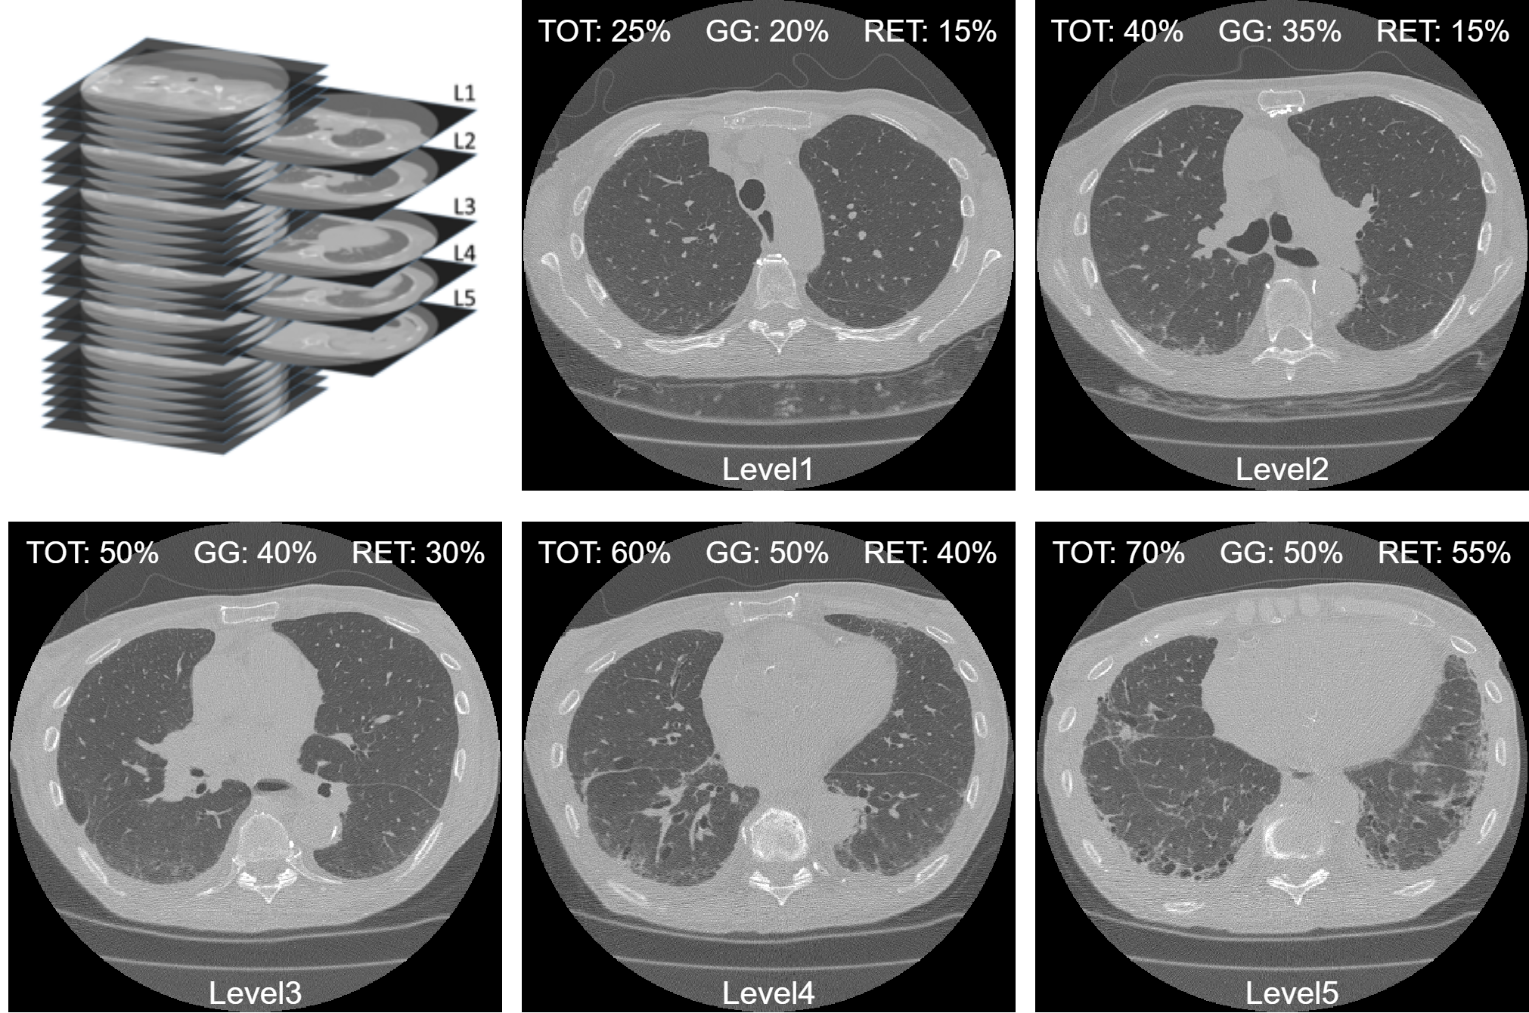
\includegraphics[width=0.8\textwidth]{figure1.png}
    \caption{Illustration of five levels in the same CT volume from one patient of systemic sclerosis. Interstitial lung disease scores from human experts are annotated on the top of each image. The level numbers are annotated at the bottom. TOT = total disease extent, GG = ground glass opacity, RET = reticular pattern.}
    \label{fig1}
\end{figure}

Nonetheless, visual scoring remains a challenging task, because of difficulties in recognizing different patterns and estimating its ratio to the whole lung. From Figure \ref{fig1} it is conceivable how difficult it is to identify different patterns and estimate their ratios for each level, especially when GG and RET overlap. Therefore, an atlas was published to provide a guiding consensus document to reduce inter-observer variability \cite{Williamson2021}. Despite this, ILD scoring is still laborious and dependent on rater experience. Therefore, an automatic scoring tool is needed to overcome these limitations \cite{Collins1994, Sverzellati2011} and to make the scoring available for clinical practice. An automated scoring tool would consist of two steps: 1) selecting the five levels (axial CT slices) according to anatomical landmarks; and 2) estimating the score for each selected slice by recognizing the different patterns and estimating their proportion to the total lung area. Recently, deep neural networks have been proposed for anatomical level localization \cite{Belharbi2017} and quantification of imaging features \cite{Chassagnon2020, GonzalezSerrano2018, Gonzalez2018}, which are closely related to the two steps needed for automated ILD scoring. While several methods combined the two steps together to estimate other imaging biomarkers \cite{Wang2017, Dabiri2020, Bridge2018, Shadmi2018}, there are few published works applied on SSc-ILD scoring. 

The purpose of this study was, therefore, to build a fully automated framework to select the five anatomical levels and score the extent of SSc-ILD for each level directly, without needing manual segmentations. The main contributions of this paper are as follows:
\begin{itemize}
  \item To the best of our knowledge, we are the first to propose aN automated framework for SSc-ILD scoring without pixel-wise fibrosis annotation. 
  \item We introduced a data synthesis method to generate training images with exact SSc-ILD scores, leading to significant improvement in the SSc-ILD scoring.
  \item We proposed replacement-based heat maps, which can visually explain the network’s output, making the framework more easily acceptable for clinicians. The reliability of heat maps was evaluated by an automatic evaluation method and by two human experts.
  \item Our framework performed competitively to experienced human experts, while costing only several seconds.
\end{itemize}


\section{Related work}

An automated scoring framework may consist of two networks: 1) level selection (i.e. localization) from 3D medical images; and 2) scoring of the resulting 2D image slices. This section therefore reviews related studies of these two topics and their application on SSc-ILD.

\subsection{Automated level selection}

Existing methods show that, despite trained on global image-level labels, convolution neural networks (CNNs) have a remarkable ability to localize objects-of-interest \cite{wei2020slir}.  Level selection aims to localize the anatomical level or anatomical landmarks \cite{Assayag2012, Goh2008} from 3D CT images. In recent years, there are a great number of works on landmark localization in 3D medical images (see Table \ref{table: rl_works}), e.g. localization of the upper and lower edge of lungs \cite{proskurov2021fast} in chest CT images, the lumbar vertebra \cite{chen2015automatic, Belharbi2017, cheng2021automatic} in spine CT images, the anatomical landmarks in cardiac ultrasound images \cite{jafari2019automatic}, anatomical structure localization in CT images \cite{de2017convnet, humpire2018efficient},  probe  localization in liver CT images \cite{wei2020slir}. The network design of these works all consist of a feature extractor followed by several fully connected layers. The feature extractors consist of several CNN blocks (a CNN layer, a normalization layer and an activation layer) with residual connections \cite{cheng2021automatic}. Although these works are all developed for non-SSc patients, the success of regression networks on the aforementioned works shows its potential on level selection of SSc patients.

\subsection{Automated scoring}

A large number of deep neural networks has been proposed for scoring tasks in general medical imaging, which were not focused on scoring SSc-ILD. An indirect method is to develop a segmentation network and score images based on lesion segmentation results, such as idiopathic pulmonary fibrosis \cite{nam2023prognostic}. The limitation of such an indirect scoring method is that it requires pixel-wise segmentation labels. A direct method is to develop a network to output the score directly without any segmentation. If the scoring output contains less than 5 categories, researchers usually treat it as a classification task, such as Gleason scoring of prostate cancer in histopathology images \cite{nagpal2019development, linkon2021deep, bulten2020automated}, grading of ulcerative colitis in endoscopic images \cite{stidham2019performance}, grading of abnormalities in knee MRI \cite{astuto2021automatic}, diabetic retinopathy grading in eye fundus images \cite{araujo2020dr}, osteoarthritis severity grading in knee MRI \cite{chen2019fully}, fibrosis estimation \cite{Walsh2022}. When the scoring is a real (floating point) number or contains more than 5 categories, regression neural networks are preferred, e.g. Agatston scoring in chest CT images \cite{cano2018automated}, ventricle function indices estimation in ultrasound images \cite{luo2020commensal}, coronary calcium scoring in chest CT scans \cite{de2019direct, mu2022calcium}, bone mineral density (BMD) and the estimation of percentage of lung emphysema from CT scans \cite{gonzalez2018deep}. Because we aimed to estimate the ratio of fibrosis to the total lung area without segmentation, a regression neural network was adopted in our work.



\begin{table}[]
\centering
\caption{Summary of related works for automated scoring frameworks on medical imaging}
\label{table: rl_works}
\begin{tblr}{
  cells = {c},
  cell{2}{1} = {r=15}{},
  cell{2}{2} = {r=5}{},
  cell{2}{3} = {r=5}{},
  cell{7}{2} = {r=10}{},
  cell{8}{3} = {r=5}{},
  cell{13}{3} = {r=4}{},
  cell{17}{1} = {r=2}{},
  cell{17}{2} = {r=2}{},
  cell{17}{3} = {r=2}{},
  hline{1-2,17,19} = {-}{},
  hline{7} = {2-5}{},
  hline{8, 13} = {3-5}{},
}

\textbf{Patients} & \textbf{Task}                          & \textbf{Network} & \textbf{Target}                 & \textbf{Dataset}     \\
Non-SSc           & localization                                 & regression       & lung upper and lower edge \cite{proskurov2021fast}       & chest CT           \\
                  &                                                 &                  & lumbar vertebra \cite{cheng2021automatic}                & spine CT           \\
                  &                                                 &                  & anatomical structures \cite{humpire2018efficient}          & body CT            \\
                  &                                                 &                  & anatomical plane landmarks \cite{jafari2019automatic}     & cardiac ultrasound \\
                  &                                                 &                  & probe localization \cite{wei2020slir}             & liver CT           \\
                  & scoring                                         & segmentation     & idiopathic pulmonary fibrosis \cite{nam2023prognostic}  & chest CT           \\
                  &                                                 & classification   & grading of ulcerative colitis \cite{stidham2019performance}  & endoscopic         \\
                  &                                                 &                  & grading of abnormalitie \cite{astuto2021automatic}         & knee MRI           \\
                  &                                                 &                  & diabetic retinopathy grading \cite{araujo2020dr}   & eye fundus         \\
                  &                                                 &                  & osteoarthritis severity grading \cite{chen2019fully} & knee MRI           \\
                  &                                                 &                  & fibrosis estiation \cite{Walsh2022}             & chest CT           \\
                  &                                                 & regression       & ventricle function indices \cite{luo2020commensal}     & cardiac ultrasound         \\
                  &                                                 &                  & coronary calcium scoring \cite{de2019direct, mu2022calcium}       & chest CT           \\
                  &                                                 &                  & percentage emphysema \cite{gonzalez2018deep}           & chest CT           \\
                  &                                                 &                  & Agatston scoring \cite{cano2018automated}               & chest CT           \\
SSc included      & scoring                                         & segmentation     & SSc-ILD assessing \cite{Chassagnon2020}                            & chest CT           \\
                  &                                                 &                  & CTD-ILD assessing \cite{su2023computed}  & chest CT           \\

                  &                                                 &                  &                                 &                    \\
                  &                                                 &                  &                                 &                    \\
                  &                                                 &                  &                                 &                    \\
                  &                                                 &                  &                                 &                    \\
                  &                                                 &                  &                                 &                    \\
                  &                                                 &                  &                                 &                    
\end{tblr}
\end{table}

\subsection{Automated scoring for SSc-ILD}
To the best of our knowledge, there are no automated level selection methods published for SSc scoring. In addition, there are only two automated scoring frameworks developed for SSc patients (see Table \ref{table: rl_works}). Chassagnon et al. \cite{Chassagnon2020} developed networks, which could output the fibrosis areas and severity quantification for SSc patients. However, their work used segmentation networks to output the pixel labels as a basis for computing the final biomarkers, which is time-consuming and requires laborious manual pixel-wise annotations for training. Since pixel-wise annotations for GG and RET are even more difficult to obtain due to unclear boundaries between the two patterns, only TOT patterns have been segmented to assess SSc-ILD. In contrast to only segmenting TOT pattern, Su et al. \cite{su2023computed} developed a severity scoring model for connective tissue disease associated ILD (CTD-ILD, including SSc-ILD) that could segment GG, RET and honeycombing patterns, separately. This also requires laborious pixel-wise annotations. As far as we know, there are no published methods on automated scoring of SSc-ILD without the need for pixel-wise fibrosis annotations.

\section{Materials and methods}
The proposed two-step framework is shown in Figure \ref{fig2}. A level selection network (L-Net) selects the five anatomical levels from the input 3D CT scans. Subsequently, five 2D slices were selected according to the five level positions and an SSc-ILD scoring network (S-Net) estimates three scores (TOT, GG and RET) for each input 2D slice.



\begin{figure}[tb]
    \centering
    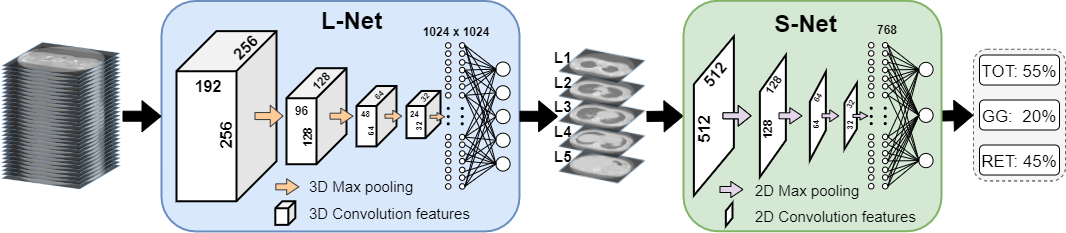
\includegraphics[width=0.8\textwidth]{figure2.png}
    \caption{Proposed framework for SSc-ILD scoring based on two cascaded neural networks. L-Net outputs five values of anatomical levels. S-Net outputs three values for automatic SSc-ILD scoring. TOT = total disease extent, GG = ground glass pattern, RET = reticular pattern.}
    \label{fig2}
\end{figure}


\subsection{Dataset}
The dataset was collected retrospectively and consisted of de-identified high-resolution CT scans of 230 SSc patients, who were referred to our multidisciplinary healthcare program \cite{Meijs2016} for suspected SSc (Table \ref{table: data}). The CT scans were performed with an Aquilion 64 scanner (Canon Medical Systems), with 120 kVp, median tube current 140 mA, median CTDIvol 8.2 mGy, rotation time 0.4 seconds, collimation $64 \times 0.5$ mm and 0.8 helical beam pitch \cite{Ninaber2015a}. Images were reconstructed with filtered back projection and using an FC86 kernel, $0.64 \times 0.64$ mm median pixel spacing, and a slice thickness and increment of 0.5 and 0.3 mm, respectively. The local Medical Ethical Committee approved the protocol, and all patients gave written informed consent. The dataset was randomly split into three groups with 135, 45 and 50 patients for training, validation and testing, respectively.

\begin{table}[]
\centering
\caption{Dataset properties of systemic sclerosis patients.}
\label{table: data}
\begin{threeparttable}
\begin{tabular}{lcc}
\hline
\textbf{Characteristic}                       & \multicolumn{2}{c}{\textbf{Patients, (n=230)}} \\ \hline
Age {[}years{]} (standard deviation)          & 54                   & (14.0)                  \\
Female (\%)                                   & 191                  & (83.0)                  \\
Interstitial lung disease detected on CT (\%) & 96                   & (41.7)                  \\
Anti-centromere antibodies positive (\%)      & 88                   & (38.3)                  \\
Anti-topoisomerase antibodies positive (\%)   & 56                   & (24.3)                  \\
Pulmonary arterial hypertension (\%)          & 8                    & (3.5)                   \\
Disease Subset:                               &                      &                         \\
\hspace*{1em}Non-cutaneous (\%)                            & 29                   & (12.6)                  \\
\hspace*{1em}Diffuse cutaneous (\%)                        & 62                   & (27.0)                  \\
\hspace*{1em}Limited cutaneous (\%)                        & 133                  & (57.8)                  \\
\hspace*{1em}Alternative diagnosis* (\%)                   & 6                    & (2.6)                   \\ \hline
\end{tabular}
\begin{tablenotes}
\item[*] Morphea scleroderma, undifferentiated connective tissue disease (UCTD), UCTD with Sjögren's syndrome, puffy fingers without systemic disease, and two cases of very early diagnosis of systemic sclerosis (VEDOSS).
\end{tablenotes}
\end{threeparttable}
\end{table}

Before training the L-Net, all CT scans were resized to a fixed size of $256 \times 256 \times 256$-pixel matrix. After resizing, the pixel spacing along the $x$ and $y$ axis was 1.26 mm. The average spacing along the z-axis was 1.2 mm. CT values were truncated between -1500 HU and 1500 HU. The world positions of five levels for each CT scan were manually selected by a rheumatologist (Observer-1, 5-year experience) and a radiologist (Observer-2, 20-year experience) in consensus. Subsequently, we converted the world positions of the five levels to relative slice numbers in the resampled 3D CT scans (the bottom slice was regarded as number 0, corresponding to the base of the lung) \cite{Jia2022}. These slice numbers were used as the ground truth. To increase the image diversity for training the L-Net, we randomly cropped patches with a fixed size of $256 \times 256 \times 192$ (ordered by $xyz$) on-the-fly during training. These patches always covered all five levels and could also be fitted into the GPU memory of 11 GB.

While L-Net was trained and tested using the down-sampled CT volumes, S-Net used the 2D axial slices of five levels with the original in-plane resolution ($512 \times 512$) from the aforementioned 230 scans. High-resolution images include fine spatial details, which can help to distinguish and grade the three fibrosis patterns. All 2D slices were scored in consensus by two experts to obtain the ground truth. Additionally, to evaluate inter/intra-observer agreement 16 patients (80 axial slices) were randomly selected from the testing dataset and the two experts scored them independently. Then they independently scored the same 80 axial slices again after six weeks. The TOT, GG and RET scores can range from 0\% to 100\%, and were estimated with a precision of five percent (Appendix Figure A1), following the protocol by Goh et al \cite{Goh2008}. To augment our dataset, two neighboring slices (above and below the chosen slice of each level) were added for training. Because the spacing of neighboring slices is only 0.3 mm, we assumed that these represent the same score. In addition, the 2D training images were augmented on the fly by random rotation ($\pm30^\circ$), scale (95\% – 105\%) and shift ($\pm$10 pixels) along the horizontal and vertical direction.

\subsection{Network design}
Inspired by \cite{Belharbi2017}, we experimented with different 3D VGG \cite{Simonyan2014} networks as the structure L-Net (Figure \ref{fig3}-A), including VGG11, VGG16 and VGG19. Deeper networks like 3D ResNet50 \cite{he2016deep} would lead to GPU memory problems with the same input patch size, so no deeper networks were tested further. Therefore, VGG11 was finally selected for L-Net. As for the S-Net, we evaluated different 2D networks with different capacities including SqueezeNet \cite{iandola2016squeezenet}, VGG11,16, and 19 \cite{Simonyan2014}, ResNet18 \cite{he2016deep}, ResNet50, ResNeXt50 \cite{xie2017aggregated}, DenseNet \cite{Huang2016}, ShuffleNet \cite{zhang2018shufflenet}, ConvNeXt \cite{Liu2022}, and finally decided to adopt ConvNeXt for S-Net due to its state of the art performance (Figure \ref{fig3}-B). Compared with the original VGG11 proposed in \cite{Simonyan2014}, L-Net extends all convolutional and max-pooling layers from 2D to 3D. The feature extractor (convolutional layers) of the S-Net was initialized by pre-trained weights from ImageNet \cite{Liu2022}, while the fully connected layers were initialized randomly using a normal distribution. The architecture and training details of L-Net and S-Net are shown in Table \ref{table: netdesign}.


\begin{figure}[tb]
    \centering
    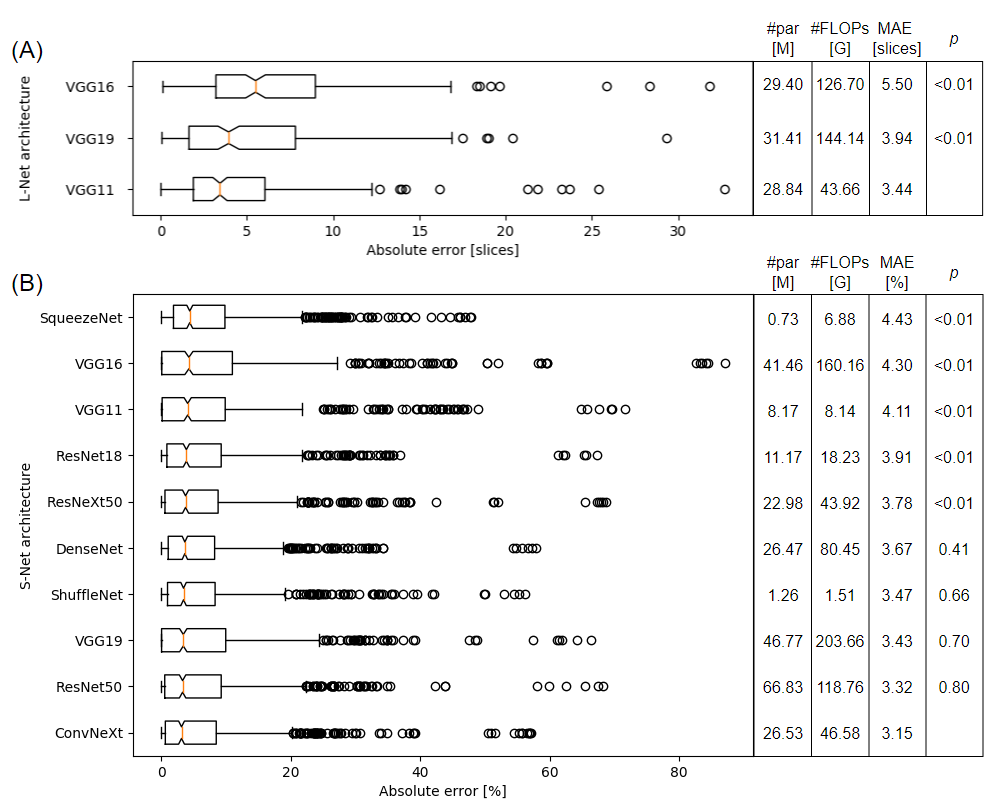
\includegraphics[width=0.8\textwidth]{figure3.png}
    \caption{Network architecture selection for L-Net (A) and S-Net (B). \#par: number of trainable parameters; \#FLOPs: number of floating point operations; MAE: mean absolute error. VGG11 and ConvNeXt achieve the lowest MAE for L-Net and S-Net, respectively. p-values in (A) were obtained by the Wilcoxon signed rank test between each network and VGG11; p-values in (B) were obtained by the Wilcoxon signed rank test between each network and ConvNeXt.}
    \label{fig3}
\end{figure}

\begin{table}[]
\centering
\caption{Details of network design and training scheme for L-Net and S-Net.}
\label{table: netdesign}
\begin{tabular}{c<{\centering}m{2cm}<{\centering}m{3cm}<{\centering}}
\hline
\centering Net                     & L-Net (VGG-11) & S-Net (ConvNeXt) \\ \hline
\centering Structure & 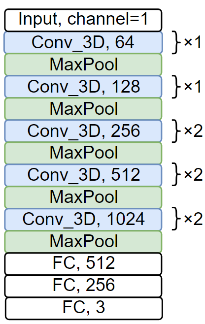
\includegraphics[width=2cm]{lnet.png}               &  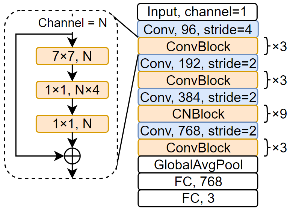
\includegraphics[width=3cm]{snet.png}                \\
\centering Dimension               & 3D             & 2D               \\
\centering Batch size              & 4              & 10               \\
\centering Training time (h)       & 2.8            & 4.9              \\
\centering Parameters (M)          & 28.84          & 22.53            \\
\centering Training epochs         & 500            & 500              \\
\centering Learning rate           & 0.0001         & 0.0001           \\ \hline
\end{tabular}
\end{table}


\subsection{Techniques to overcome label imbalance}
From Appendix Figure A1, we could find that the score distribution is highly askew—some high scores even do not exist in training dataset. The noticeable score imbalance with 50\% of TOT scores being 0 would limit the networks’ performance. Therefore, to ensure a balanced score distribution during training, we developed a sampling method that randomly selects training images with a probability inversely proportional to the ratio of each TOT score \cite{zhang2019balance}. In this way, the scores that appear less frequently (i.e. higher scores) would be used for training more frequently. To further address the label imbalance and to increase data diversity, we synthesized training images with SSc-ILD scores that are lacking in the original dataset, by digitally inserting GG and RET patterns into healthy training images.



\begin{figure}[tb]
    \centering
    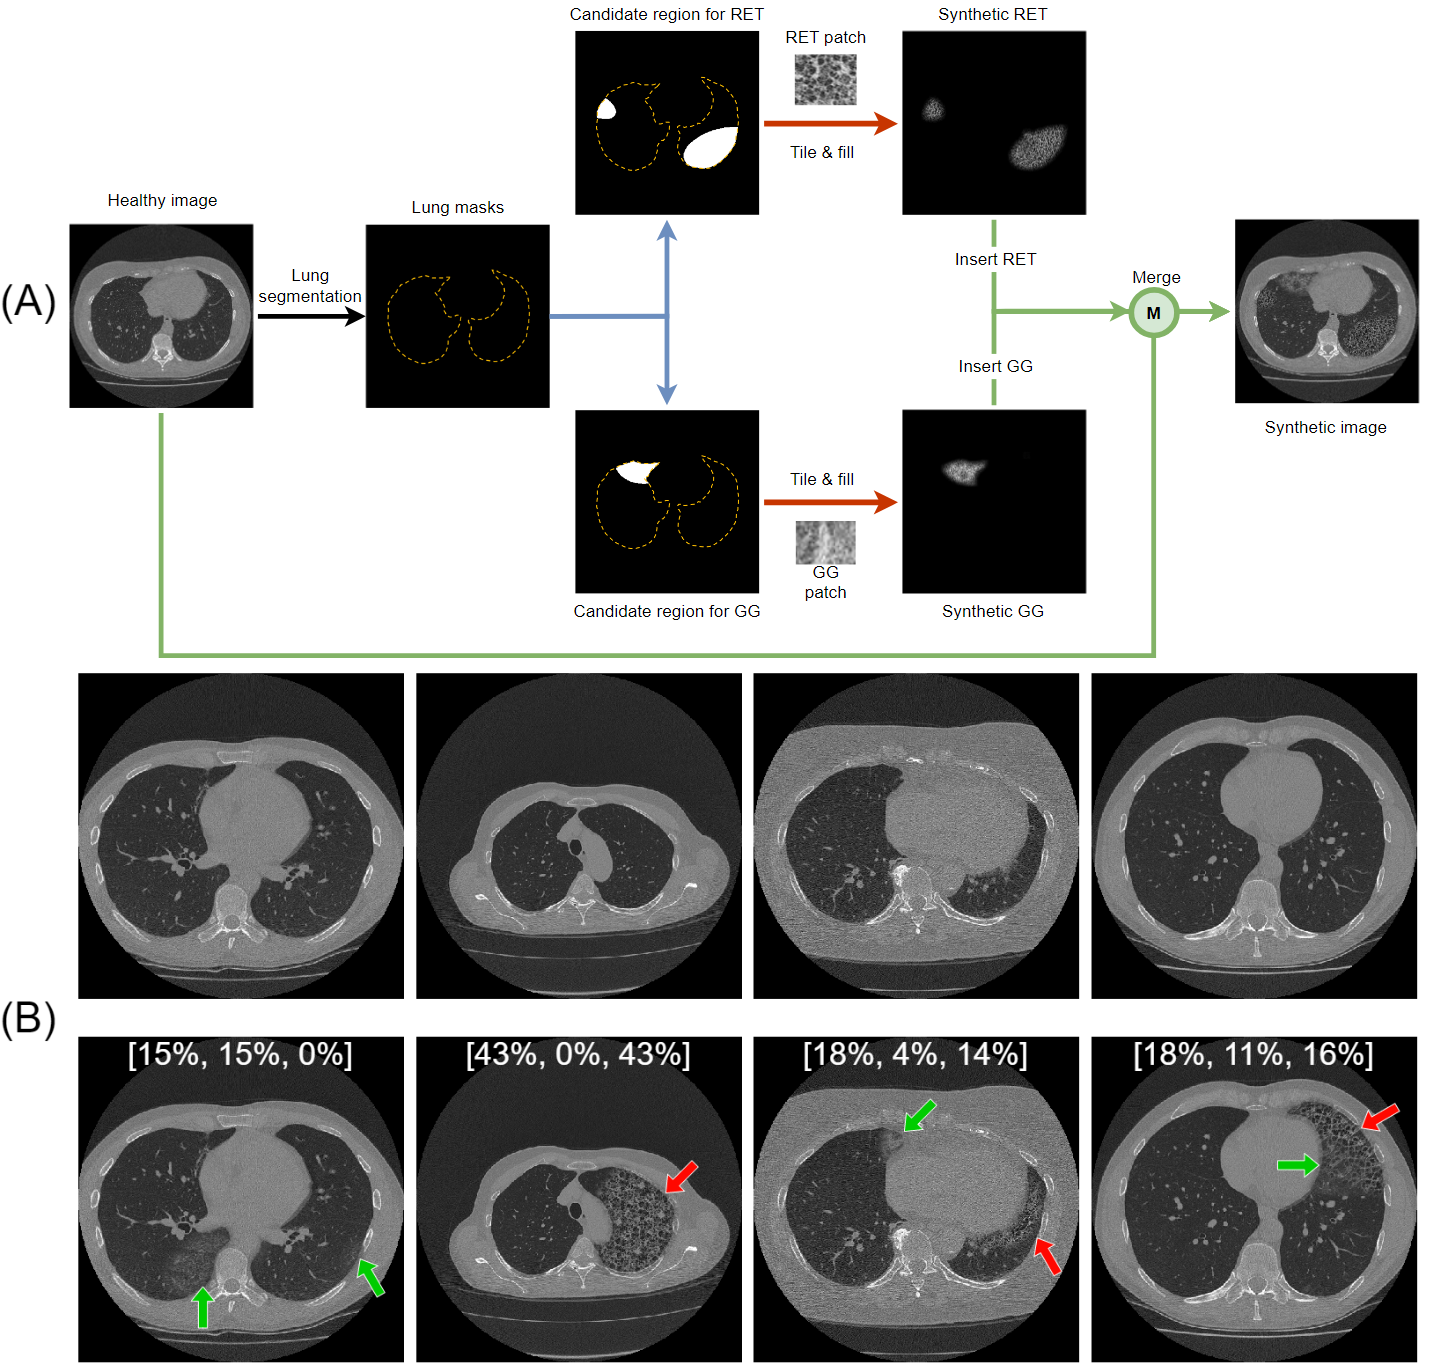
\includegraphics[width=0.8\textwidth]{figure4.png}
    \caption{Data synthesis flowchart and examples. (A) Flowchart to synthesize images with different disease patterns. Blue arrows indicate the generation of random candidate lesion regions; blue arrows indicate the generation of candidate regions, red arrows indicate the filling of patterns; green arrows indicate the insertion of patterns. (B) Four pairs of synthetic examples. The upper row shows the original images; the lower row shows the corresponding synthetic images. Green arrows point to GG; red arrows point to RET. Different pattern combinations are shown from left to right: only GG, only RET, GG and RET without overlap, GG and RET with overlap. The scores of these synthetic images are shown on the image in the order of [TOT, GG, RET]. TOT = total disease extent, GG = ground glass pattern, RET = reticular pattern.}
    \label{fig4}
\end{figure}


The flowchart of data synthesis is shown in Figure \ref{fig4}-A. First, we created two patches full of different patterns, one for GG and one for RET, by manually extracting local CT patches from training images with high scores in these two patterns separately. Subsequently, the healthy training images (TOT=0) were augmented by the digital insertion of these patterns. The candidate lesion regions for the pattern insertion were randomly generated by defining up to three ellipses with random centers, orientations and axes lengths (lengths range from 1 to 150 pixels), which were then cropped by the lung mask to ensure the patterns will be inserted in the lung area only. The lung mask was automatically generated by a multi-atlas based automatic lung segmentation algorithm \cite{Zhai2019}. To avoid introducing unrealistic borders during pattern insertion, the inserted patterns gradually fade out at the edge, by a Gaussian decay in intensity. To increase the pattern diversity of synthetic data, we always applied random rotation ($\pm180^\circ$) and scale (95\%–105\%) to the patterns before each pattern insertion. The disease severity scores were then adapted according to the area of inserted patterns. Some synthetic image examples and their scores were shown in Figure \ref{fig4}-B. The synthetic data constitute half of the training dataset, while validation and testing were performed on real patient data only.

\subsection{Heat map visualization: network explainability}
Application in clinical practice is limited, if the output of a deep learning network is difficult to explain. Therefore, inspired by the occlusion-based visualization method \cite{zeiler2014visualizing}, we developed a replacement-based method to generate heat maps, indicating which areas were important for the S-Net in recognizing different disease patterns. The method details are as follows.


\begin{figure}[tb]
    \centering
    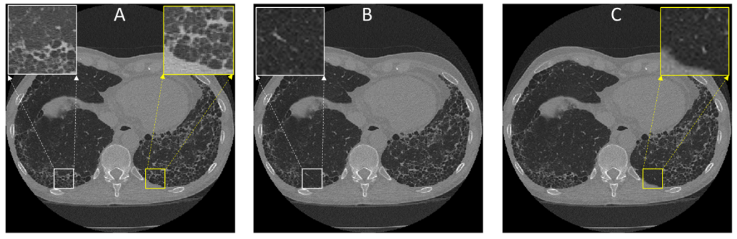
\includegraphics[width=0.8\textwidth]{figure5.png}
    \caption{Illustration of the replacement-based heat map. (A) Original CT slice. (B) A patch in the lung is replaced by a healthy patch. (C) A patch at the edge of the lung is replaced by a healthy patch while the pixels outside the lung were kept unchanged.}
    \label{fig5}
\end{figure}

A rectangular patch full of healthy lung tissue, in advance cropped from a lung region of healthy slices, was used to cover the test image from top-left to bottom-right step-by-step, separately. The patch size was $64 \times 64$ pixels with a step size of 16. Two examples of the replaced images are shown in Figure \ref{fig5}.  The output score from the S-Net of the original test image was regarded baseline. Each time we slide the healthy patch, the original image was occulted by the healthy patch at a different position. We could obtain the new score from S-Net and record its change at each position. A heat map of the image is then generated using the magnitude of the score change ($\Delta P$). A negative score change ($\Delta P<0$) implies that the network regarded the original patch as diseased since the score decreased after concealing the area with healthy tissue. If the output score remains unchanged ($\Delta P=0$), the original patch was already considered healthy. A score increase ($\Delta P>0$) means that the network produced a false positive, since the inserted healthy patch was apparently classified as diseased. To make sure that the replaced pixels are in the lung area, the rectangular healthy patch was cropped by the lung mask before each replacement (Figure \ref{fig5}-C). The patch edge fades gradually by linearly increasing transparency to make it more natural.

This replacement-based heat map was inspired by the occlusion-based visualization method \cite{zeiler2014visualizing}. The difference is that the occlusion-based method would cover the original image using a patch with a constant value, which would introduce artifacts, while our replacement-based method covers the original image using a patch cropped from a healthy CT scan, which still includes lung texture and makes the generated image more natural. 

In order to evaluate the performance of the heat maps, blinded to the network’s output, two human experts independently rated their agreement with the heat maps using a Likert scale, with five labels (1-5): “Strongly disagree”, “Disagree”, “Neutral”, “Agree” and “Strongly agree”, using dedicated software (Appendix Figure A2).

Additionally, we developed an automatic method to evaluate the heat map’s explainability. By thresholding the heat map, the different patterns were segmented and their areas were divided by the total lung area, to obtain a derived SSc-ILD score. Subsequently, we tested the network’s consistency by the correlation between the derived SSc-ILD score and the network’s output. The optimal threshold was obtained from the validation dataset by varying the threshold from -4\% to 0\% and selecting the one with the smallest mean absolute error (MAE) between the derived SSc-ILD score and S-Net output.

\subsection{Statistical analysis and evaluation}
To evaluate our networks, the following statistical analyses were performed by an in-house Python 3.8 script with corresponding libraries.

The mean absolute error (MAE), standard deviation (STD) and 95\% confidence intervals (CI) are reported. To evaluate the inter-observer agreement, Cohen’s linearly weighted kappa ($\kappa$) \cite{Koo2016} and intra-class correlation coefficient (ICC) [36] were used. $\kappa$ was calculated by scikit-learn 0.24.2 \cite{Pedregosa2011}. ICC was calculated by pingouin 0.4.0 \cite{Vallat2018} based on a single-rating, absolute-agreement, 2-way mixed-effects model \cite{Koo2016}. To statistically test differences between groups, a paired T-test and Wilcoxon signed rank test were performed, as implemented by scikit-learn 0.24.2. A P value of less than 0.05 was considered to indicate a statistically significant difference. All metrics were calculated based on the testing dataset unless stated otherwise.

\subsection{Network implementation details}
Our neural networks, L-Net and S-Net, were implemented using PyTorch 1.7.1 (\url{https://pytorch.org}). For both networks, the loss function was the mean squared error (MSE). The Adam optimizer was used with a learning rate of 1e-4, a weight decay of 1e-4 and 500 epochs. Multithreading was used to accelerate the on-the-fly data augmentation. The workstation for training and validation was equipped with an Intel(R) Xeon(R) CPU Gold 6126 @ 2.6GHz with 90 GB memory and a GPU RTX 2080TI with 11 GB memory. The source code and trained models are published at \url{https://github.com/Jingnan-Jia/ssc_scoring} to facilitate  reproduction of results.


\section{Experiments and results}

\subsection{SSc-ILD scoring performance}
First, we trained and evaluated the L-Net (Figure \ref{fig6}) and S-Net (Table \ref{table: tb3}), separately. Subsequently, an end-to-end framework was built as a cascade of the trained L-Net and S-Net (called L\&S-Net), in which the input slices for S-Net were automatically selected by the L-Net (Table \ref{table:tb4}). For none of the levels, the automatic scoring results of L\&S-Net showed any significant differences as compared to solely S-Net which received the manually selected slices (Table \ref{table:tb4}).


\begin{figure}[tb]
    \centering
    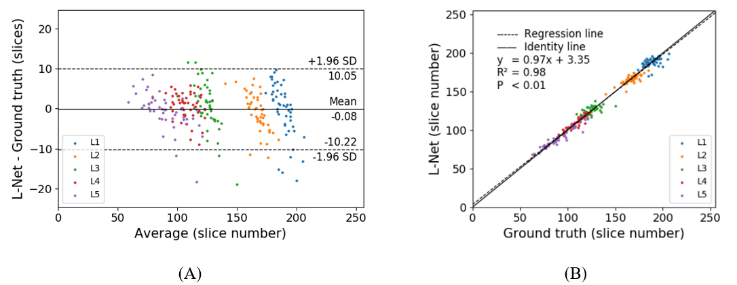
\includegraphics[width=0.8\textwidth]{figure6.png}
    \caption{Testing results of the L-Net in selecting slices on the five levels, L1–L5. (A) Bland-Altman plot and (B) Correlation plot. The average spacing between slices was 1.2 mm. The ICC of the five consecutive levels was 0.72, 0.84, 0.81, 0.96 and 0.97. No significant bias was observed among the five levels (P=0.20, 0.93, 0.42, 0.49, and 0.76, respectively).}
    \label{fig6}
\end{figure}

\begin{table*}
\centering
\caption{SSc-ILD scoring performance from S-Net with different technique combinations.}
\label{table: tb3}
\begin{threeparttable}
\begin{tblr}{
  cells = {c},
  cell{1}{5} = {c=3}{},
  cell{1}{8} = {c=3}{},
  cell{1}{11} = {c=3}{},
  vline{5-6,9} = {1}{},
  vline{5,8,11} = {2-10}{},
  hline{1-4,7,10-11} = {-}{},
}
\textbf{Experiments} & \textbf{DS*} & \textbf{BS} & \textbf{PT} & \textbf{TOT} &           &      & \textbf{GG}  &           &      & \textbf{RET} &           &      \\
(i)                  &              &             &             & MAE [\%]↓    & $\kappa$↑ & ICC↑ & MAE [\%]↓    & $\kappa$↑ & ICC↑ & MAE [\%]↓    & $\kappa$↑ & ICC↑ \\
                     & -            & -           & -           & 8.87 (12.55) & 0.42      & 0.59 & 6.62 (11.64) & 0.31      & 0.38 & 6.59 (9.30)  & 0.42      & 0.58 \\
                     & -            & -           & \ding{51}          & 7.85 (10.71) & 0.53      & 0.72 & 5.96 (10.03) & 0.45      & 0.60 & 5.81 (8.42)  & 0.53      & 0.72 \\
(ii)                 & -            & \ding{51}          & -           & 8.30 (11.35) & 0.46      & 0.62 & 5.89 (10.88) & 0.40      & 0.48 & 5.96 (8.70)  & 0.48      & 0.65 \\
                     & \ding{51}           & -           & -           & 6.74 (9.59)  & 0.59      & 0.77 & 5.07 (9.38)  & 0.54      & 0.67 & 5.08 (7.76)  & 0.57      & 0.75 \\
                     & -            & \ding{51}          & \ding{51}          & 6.87 (9.61)  & 0.59      & 0.77 & 5.09 (9.50)  & 0.54      & 0.66 & 5.11 (7.45)  & 0.59      & 0.78 \\
(iii)                & \ding{51}           & \ding{51}          & -           & 7.98 (11.31) & 0.48      & 0.64 & 5.43 (9.82)  & 0.47      & 0.60 & 5.52 (8.56)  & 0.52      & 0.69 \\
                     & \ding{51}           & -           & \ding{51}          & 6.26 (8.67)  & 0.63      & 0.82 & 4.76 (8.81)  & 0.58      & 0.70 & 4.76 (6.70)  & 0.62      & 0.82 \\
(iv)                 & \ding{51}           & \ding{51}          & \ding{51}          & 5.90 (8.77)  & 0.66      & 0.83 & 4.66 (8.83)  & 0.58      & 0.71 & 4.49 (6.70)  & 0.65      & 0.84 
\end{tblr}
\begin{tablenotes}
\item[*] DS = Data synthesis, BS = Balanced sampling, PT = Pre-training, TOT = total disease extent, GG = ground glass pattern, RET = reticular pattern, Mean absolute error (MAE) is followed by the standard deviation (STD) between parentheses, $\kappa$ = Cohen’s weighted kappa, ICC = Intra-class correlation coefficient. ↓ = lower is better, ↑ = higher is better. Bold numbers indicate the best performance. (i). Baseline established by training the S-Net from scratch without balanced sampling or synthesized data. (ii). Introducing either pre-trained weights from ImageNet, balanced sampling or data synthesis. (iii). Combination of two of the three techniques. (iv). Combination of all three techniques which obtained the best performance. Therefore, the proposed method contains all three techniques.
\end{tablenotes}
\end{threeparttable}
\end{table*}



% 
\begin{table*}
\centering
\caption{MAE comparison of SSc-ILD scoring between the whole framework (L\&S-Net) and sole S-Net.}
\label{table:tb4}
\begin{threeparttable}
\begin{tblr}{
  cells = {c},
  cell{1}{1} = {r=2}{},
  cell{1}{2} = {c=3}{},
  cell{1}{5} = {c=3}{},
  cell{1}{8} = {c=3}{},
  hline{1,3,9} = {-}{},
}
Level & MAE of TOT*          &              &      & MAE of GG           &              &      & MAE of RET         &             &      \\
      & LS-Net [\%]  & S-Net [\%]   & P    & LS-Net [\%]  & S-Net [\%]   & P    & LS-Net [\%] & S-Net [\%]  & P    \\
1     & 4.20 $\pm$ 7.94  & 6.28 $\pm$ 11.57 & 0.33 & 2.34 $\pm$ 6.88  & 2.81 $\pm$ 6.71  & 0.57 & 3.49 $\pm$ 6.25 & 5.14 $\pm$ 9.67 & 0.42 \\
2     & 4.61 $\pm$ 6.89  & 4.74 $\pm$ 7.46  & 0.06 & 3.11 $\pm$ 7.67  & 3.33 $\pm$ 7.62  & 0.88 & 3.35 $\pm$ 5.67 & 3.72 $\pm$ 6.15 & 0.49 \\
3     & 5.61 $\pm$ 8.00  & 6.17 $\pm$ 8.63  & 0.64 & 4.65 $\pm$ 8.42  & 4.82 $\pm$ 8.19  & 0.56 & 4.33 $\pm$ 5.24 & 4.69 $\pm$ 6.13 & 0.74 \\
4     & 7.12 $\pm$ 8.87  & 6.88 $\pm$ 9.23  & 0.17 & 5.88 $\pm$ 9.58  & 5.98 $\pm$ 9.59  & 0.10 & 4.99 $\pm$ 6.75 & 4.93 $\pm$ 6.65 & 0.90 \\
5     & 8.12 $\pm$ 10.00 & 7.58 $\pm$ 9.99  & 0.11 & 7.13 $\pm$ 10.49 & 6.75 $\pm$ 10.41 & 0.40 & 6.15 $\pm$ 8.26 & 5.74 $\pm$ 7.78 & 0.11 \\
ALL   & 5.86 $\pm$ 8.46  & 5.90 $\pm$ 8.77  & 0.21 & 4.56 $\pm$ 8.80  & 4.66 $\pm$ 8.83  & 0.13 & 4.40 $\pm$ 6.55 & 4.49 $\pm$ 6.70 & 0.28 
\end{tblr}
\begin{tablenotes}
\item[*] Mean absolute error (MAE) $\pm$ standard deviation (STD) is presented expressed as \%, TOT = total disease extent, GG = ground glass pattern, RET = reticular pattern, ALL = Calculated based on the results from all the five levels.
\end{tablenotes}
\end{threeparttable}
\end{table*}



\subsection{Comparison with human experts}
The inter- and intra-observer agreement in the sub-group of 16 patients (80 axial slices) from the testing dataset were compared with our proposed method (Table \ref{table: tb5}). The inter-observer agreement was higher during the second scoring session. The intra-observer agreement of Observer-2 was higher than Observer-1, and the inter- and intra-observer agreement in GG scoring was always lower than in TOT and RET scoring.

For scoring TOT, our automatic method was close to the first rating by Observer-1 ($\text{Obs1}_{\text{T1}}$), but Observer-2 was closer to the consensus than our method. For GG the model had a fair agreement with human consensus, while the observers agreed moderately, and for RET the model’s agreement was moderate, but moderate/substantial for observers. Except for the second GG scoring by Observer-2 ($\text{Obs2}_{\text{T2}}$, P < 0.05), other human observations did not perform significantly better than our method. The Bland-Altman plots (Appendix Figure A3) illustrate the performance of an individual human score ($\text{Obs2}_{\text{T2}}$) and our automatic network.  

The average time of fully automated scoring for the five levels is less than ten seconds per patient, while human experts need around ten minutes (around 2.5 minutes to identify five levels and another 7.5 minutes to score three patterns of five levels).

% \usepackage{tabularray}
\begin{table*}
\centering
\caption{SSc-ILD scoring performance of human experts (Observer-1 and Observer-2) in two scoring sessions (T1 and T2, with 6 weeks interval) and our proposed network in a subset of 16 patients from the testing dataset.}
\label{table: tb5}
\begin{threeparttable}
\begin{tblr}{
  cells = {c},
  cell{1}{1} = {r=2}{},
  cell{1}{2} = {r=2}{},
  cell{1}{3} = {c=3}{},
  cell{1}{6} = {c=3}{},
  cell{1}{9} = {c=3}{},
  cell{3}{1} = {r=2}{},
  cell{5}{1} = {r=2}{},
  cell{7}{1} = {r=5}{},
  hline{1,3,5,7,12} = {-}{},
}
\textbf{Agreement}                    & \textbf{Comparison} & \textbf{TOT}*        &              &               & \textbf{GG}         &              &               & \textbf{RET}        &              &               \\
                                      &                     & \textbf{MAE [\%] ↓} & \textbf{$\kappa$ ↑} & \textbf{ICC↑} & \textbf{MAE [\%] ↓} & \textbf{$\kappa$ ↑} & \textbf{ICC↑} & \textbf{MAE [\%] ↓} & \textbf{$\kappa$ ↑} & \textbf{ICC↑} \\
{Inter-\\ observer}                   & $\text{Obs1}_{\text{T1}}$ vs $\text{Obs2}_{\text{T1}}$    & 5.25                & 0.59         & 0.76          & 4.00                & 0.54         & 0.66          & 3.81                & 0.61         & 0.82          \\
                                      & $\text{Obs1}_{\text{T2}}$ vs $\text{Obs2}_{\text{T2}}$    & 4.25                & 0.67         & 0.88          & 3.94                & 0.58         & 0.80          & 3.44                & 0.63         & 0.86          \\
{Intra-\\ observer}                   & $\text{Obs1}_{\text{T1}}$ vs $\text{Obs1}_{\text{T2}}$    & 4.38                & 0.63         & 0.83          & 3.50                & 0.56         & 0.73          & 3.06                & 0.67         & 0.84          \\
                                      & $\text{Obs2}_{\text{T1}}$ vs $\text{Obs2}_{\text{T2}}$    & 3.50                & 0.74         & 0.89          & 3.69                & 0.62         & 0.74          & 2.69                & 0.72         & 0.90          \\
{Comparison with\\ ground truth (GT)} & $\text{Obs1}_{\text{T1}}$ vs GT        & 7.06 (0.41)         & 0.51         & 0.73          & 5.63 (0.51)         & 0.44         & 0.68          & 4.94 (0.37)         & 0.56         & 0.76          \\
                                      & $\text{Obs1}_{\text{T2}}$ vs GT        & 6.19 (0.14)         & 0.58         & 0.82          & 5.38 (0.78)         & 0.46         & 0.59          & 4.75 (0.13)         & 0.58         & 0.78          \\
                                      & $\text{Obs2}_{\text{T1}}$ vs GT        & 6.56 (0.42)         & 0.58         & 0.80          & 5.38 (0.32)         & 0.48         & 0.63          & 4.63 (0.18)         & 0.61         & 0.84          \\
                                      & $\text{Obs2}_{\text{T2}}$ vs GT        & 4.94 (0.40)         & 0.67         & 0.86          & 4.94 (0.001)$\dag$       & 0.55         & 0.75          & 4.19 (0.18)         & 0.63         & 0.80          \\
                                      & L\&S-Net vs GT        & 6.40                & 0.54         & 0.79          & 6.13                & 0.39         & 0.55          & 4.44                & 0.61         & 0.84          
\end{tblr}
\begin{tablenotes}
\item[*] TOT = total disease extent, GG = ground glass pattern, RET = reticular pattern, GT = Ground truth (human consensus score), MAE = mean absolute error, $\kappa$ = Cohen’s weighted kappa, ICC = Intra-class correlation coefficient. Data between parentheses are P values from the Wilcoxon signed rank test comparing observers with our proposed method. $\text{Obs1}_{\text{T1/T2}}$ and $\text{Obs2}_{\text{T1/T2}}$ denote the observations from Observer-1 and Observer-2 at the first or second scoring session, respectively. 
\item[\dag] Significantly better than our method (P<0.05).
\end{tablenotes}
\end{threeparttable}
\end{table*}


\subsection{Heat map explanation and its evaluation}
The replacement-based heat maps of the automatic scoring for the three different patterns are shown in Figure \ref{fig7} of different patients from the testing subset. The proposed visualization method can show areas of different patterns and display the severity with different colours. The yellow and red areas in the heatmaps (Figure \ref{fig7}) denote the negative score change after the area has been covered by a healthy patch, which means that the original patch is "diseased". A red area means more severe and more obvious patterns than a yellow area. The green and blue areas mean that the network produced a false positive, since the inserted healthy patch was apparently classified as diseased. The heat maps can also help to find the cause of errors, as shown in the last row in Figure \ref{fig7}, where the GG scoring result (30\%) is far lower than the ground truth (90\%). From the heat maps, we can see only about 30\% of the whole lung was activated (yellow and red area) and the GG pattern was missed in around 1/3 of the right lung (blue area). Alternative heat maps are presented in Appendix Figure A4 to indicate false negatives and positives.



\begin{figure}[tb]
    \centering
    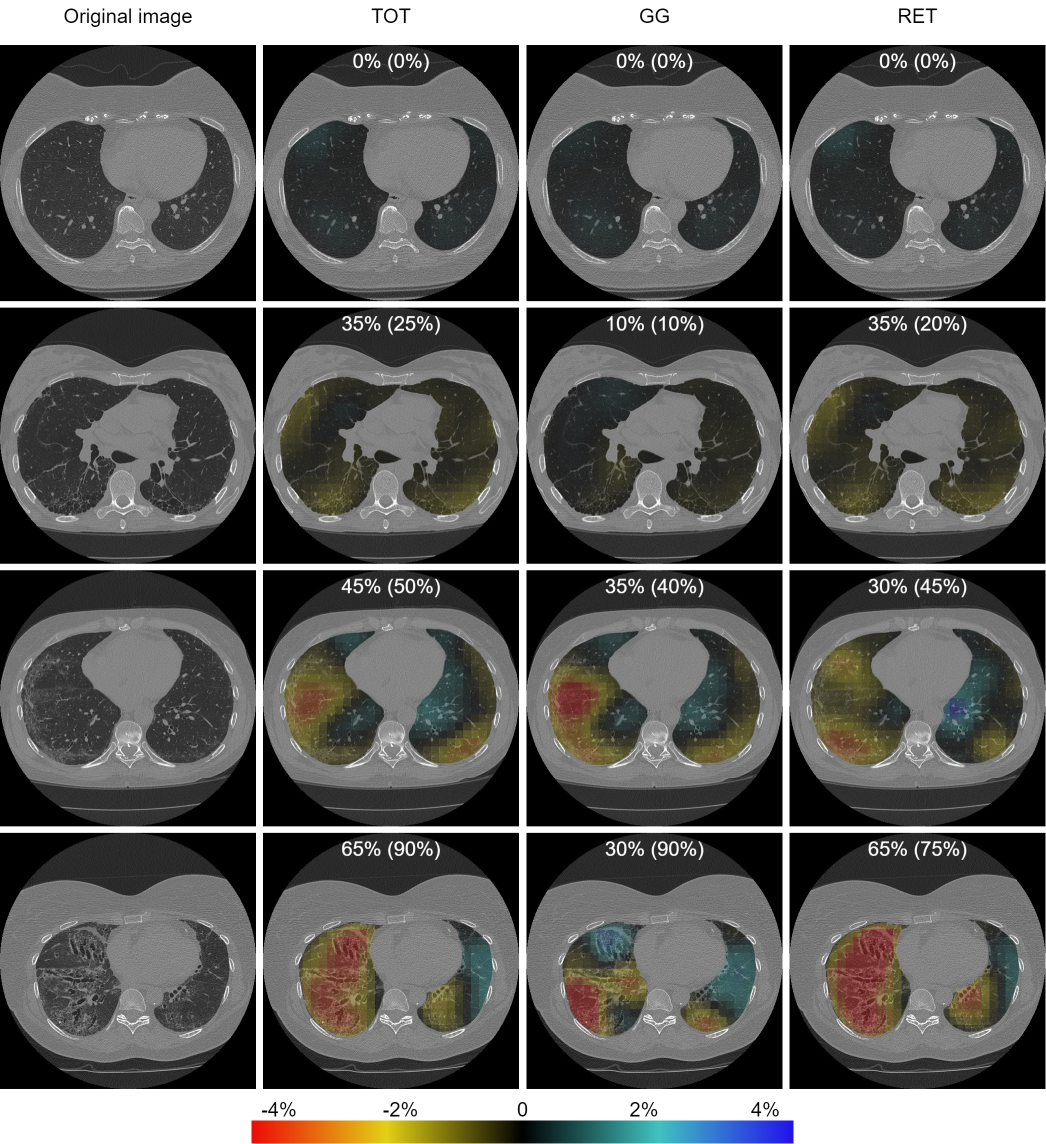
\includegraphics[width=0.8\textwidth]{figure7.png}
    \caption{Heat map visualization for various test images. Each row represents one axial slice from a different patient. The first column is the original image and the subsequent three columns show the heat maps of the three disease patterns. Different colours represent the magnitude of score change.  From top to bottom, the images show increasing disease severity. The automatic ILD score is shown on the top of each image followed by the ground truth (human consensus) between parentheses. TOT = total disease extent, GG = ground glass pattern, RET = reticular pattern.}
    \label{fig7}
\end{figure}

From the semi-quantitative evaluation of the heat maps, Observer1 rated the heat maps with “Strongly Agree” or “Agree” in 97.0\%, 94.2\% and 89.8\% of cases for TOT, GG and RET, respectively (Figure \ref{fig8}, upper row). Ratings of “Strongly agree” or “Agree” by Observer2 occurred in 84.0\%, 85.8\% and 70.2\% of cases for TOT, GG and RET, respectively. Thus, on average they agreed in 90.5\%, 90.0\% and 80.0\% with the heat maps, respectively.

After applying an optimized threshold value (Appendix Figure A5) to the heat maps on the testing dataset, a significant linear correlation was found between the heat map-derived SSc-ILD score and the L\&S-Net’s output (Figure \ref{fig8}, lower row). For TOT, GG and RET, 84\%, 87\% and 83\% of the S-Net’s output variation can be explained by the heat maps, respectively.


\begin{figure}[tb]
    \centering
    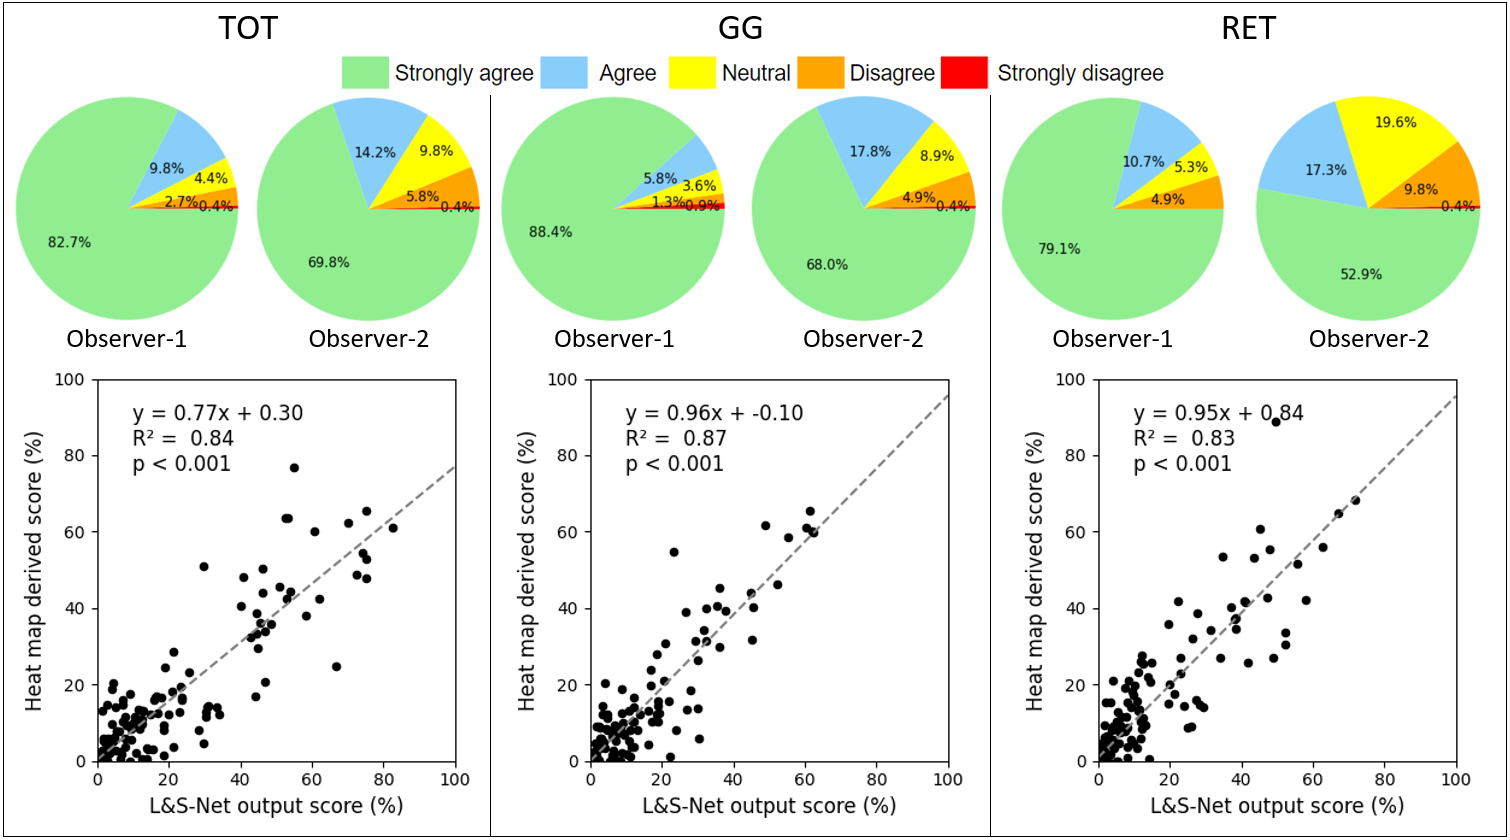
\includegraphics[width=0.8\textwidth]{figure8.png}
    \caption{eat map performance evaluated by the two observers (pie charts in the upper row) and the association between the heat map derived ILD scoring and L\&S-Net’s output (scatter plots in the lower row), to indicate its explainability. TOT = total disease extent, GG = ground glass pattern, RET = reticular pattern.}
    \label{fig8}
\end{figure}

\section{Discussion}
In this study, we developed a deep learning framework to perform fully automated SSc-ILD scoring in chest CT scans. By cascading two separate networks, the framework was able to select the five anatomical levels from 3D CT scans and then quantify the extent of three different disease patterns for each level. The training of the framework only needs visual scores as the ground truth without the requirement of prior manual segmentations. Heat maps can intuitively explain the network’s output, and can be used to derive coarse segmentations of the different patterns that are consistent with the network’s output. Our framework has the potential to serve as an alternative to visual SSc-ILD scoring of lung involvement in systemic sclerosis.

\subsection{Comparison to related work}
Our work shows the feasibility to select the positions of five scoring levels and estimate the percentage of radiological patterns using regression neural networks. This provides the possibility to automate other pattern-percentage based scoring systems \cite{Assayag2012, Goldin2008, Pandey2010}. To the best of our knowledge, this is the first fully automated quantification of SSc-ILD without pixel-wise annotation. In addition to manual scoring method, the two most recent and relevant deep learning based scoring methods are shown in Table \ref{table: tb6}, which segmented SSc-ILD on CT scans to quantify the severity of disease \cite{Chassagnon2020, su2023computed}. Compared with their approach, with a similar number of patients, there are three main differences. First, our two-step framework consists of a 3D level selection network and a 2D scoring network, while they assumed that slices were already manually selected beforehand and only proposed a 2D network for lesion segmentation. Second, our score regression network just need image-wise scores for training, while their segmentation-based score assessment requires time-consuming pixel-wise annotations, which is more difficult to obtain. Third, our framework can score SSc-ILD in 10 seconds while other manual or semi-automated methods require more time.

\begin{sidewaystable}
\centering
\caption{Comparison between different methods for SSc-ILD scoring.}
\label{table: tb6}
\begin{threeparttable}
\begin{tblr}{
  cells = {c},
  row{1} = {b},
  hline{1-2,6} = {-}{},
}
\textbf{Method}                   & {\textbf{Method}\\\textbf{description}}                   & \textbf{Label} & {\textbf{Labelling }\\\textbf{ difficulty}} & {\textbf{Number of}\\\textbf{patients}} & \textbf{MAE [\%]} & \textbf{Time } \\
Manual                            & Manual slice selection + manual scoring       & NA*             & NA                                          & NA      & 7.06 to 4.19      & 10 minutes                                        \\
Segmentation-based \cite{Chassagnon2020}                & Manual slice selection + automatic scoring    & Pixel-wise    & Difficult                                   & 208               & NA                & 3 minutes   \\
Segmentation-based \cite{su2023computed}                & Manual slice selection + automatic scoring    & Pixel-wise    & Difficult                                   & 298               & NA                & 3 minutes      \\                          
Ours (regression-based)  & Automatic slice selection + automatic scoring & Image-wise     & Easy                                        & 230      & 6.40 to 4.44      & 10 seconds                                          
\end{tblr}
\begin{tablenotes}
\item[*] NA: not applicable, MAE: mean absolute error,  Time: estimated scoring time per patient, TOT = total disease extent, GG = ground glass pattern, RET = reticular pattern, HC = honeycombing.
\end{tablenotes}
\end{threeparttable}
\end{sidewaystable}


\subsection{Explanation and discussion on results}
Our framework consists of two networks, trained independently: L-Net for automatic level selection and S-Net for automatic ILD scoring. For the L-Net, the selection of the first level is more difficult (ICC = 0.72) than other levels because indicating the origin of the great vessels is variable as it was not defined precisely. Nevertheless, the automatically selected levels were accurate enough, because the ultimate scoring did not show significant differences compared with the single S-Net’s performance with manually annotated slices. This may be due to the fact that disease patterns appear and disappear only gradually from one slice to the other.

In our paper we demonstrated that different network structures with different capacities did not necessarily show a significant difference (see Figure \ref{fig3}). That implies that network design is not the bottleneck for our task. Our further investigation showed that the key issue, hindering the network performance, is the low quality of dataset. Therefore, we improved the training method by introducing synthetic training images that significantly improved the network’s performance.

For the ILD scoring network, the pre-trained weights, balanced sampling and the proposed data synthesis all helped to steadily improve the network’s performance for all three patterns. Our random ILD insertion method is very effective and easy to implement, which only requires two small patches fully covered by GG and RET. Generally, ILD in SSc has a specific distribution, e.g. classical subpleural sparing earlier in the disease \cite{Herzog2014}, which was not simulated by our synthesis method. The scoring results were however not affected by this limitation, since the neural network only needs to estimate the ratio of ILD, irrespective of the location of ILD. Nevertheless, there is still some space for improvement in GG scoring. Also for human experts, GG is more difficult to define and identify than RET patterns, because of the limited spatial resolution of CT and consequential ‘partial volume’ effect. Moreover, some GG patterns resemble noise from image acquisition or reconstruction. Conversely, reticular lesions are larger than voxel size and can be visually or automatically identified as structures, such as thickened interlobular septa or thickened airways causing pathological reticular patterns. Our proposed network may help in distinguishing noise from actual pathological ground glass lesions when noise patterns can be identified. 

With the help of the replacement-based heat map, we visualized which areas contribute to which scores respectively. Two experts evaluated the heat maps independently and both gave very satisfactory ratings. After we applied a threshold to the heat map, the ratio of different patterns to the total lung area was consistent with the automatic ILD scores by L\&S-Net. The quantitative measurement shows that our proposed heat maps can accurately explain the L\&S-Net’s output. This can increase the clinicians’ confidence in the network’s output. A heat map “highlights” the detected pathology that may help the physician with a quick image interpretation. Exploring the heat map can also be used to check the quality of the automatic score. The heat map could be regarded as a coarse segmentation of TOT, GG and RET. Normally it is not practical to have large datasets of SSc ILD pattern segmentations because it is very time-consuming and laborious. The heat maps can act as an initial step to obtain manual segmentation reducing annotation time. From this perspective, we successfully obtained a coarse ILD pattern segmentation network for SSc patients without the requirement of a segmentation ground truth. Compared with the normal binary segmentation \cite{Chassagnon2020}, the advantage of our heat map is that it also gives an indication of the severity of a disease pattern, as shown by the colour, instead of a binary classification into either healthy or disease. 

We observed that human experts gave higher ratings to the GG heat maps than RET, although the MAE of automatic GG scoring was actually consistently higher than RET. This can be explained by the fact that human experts have more confidence in recognizing RET patterns, so they use more strict criteria for RET heat maps. Since they were less confident in their GG recognition, reflected by the lower inter-/intra-observer agreement, this resulted in more tolerance for GG heat maps.

In the visual ILD scoring system, the use of only five anatomical levels has been a compromise, for clinical practice. It is already very time-consuming and laborious to manually select the five levels and score three patterns for each level (taking around ten minutes). Our method, however, could automatically complete the level selection and ILD scoring in several seconds. In addition, our method can be easily extended to score all slices of the entire CT volume, which is practically not feasible for humans.

\subsection{Limitation}
Our method has some limitations. The L-Net was initialized with a random distribution instead of pre-trained weights. This may be improved if pre-trained weights from a large 3D medical image dataset are available. The quality of data synthesis could clearly be improved further. The current pattern insertion method may distort the structure of airways and vessels and introduce some periodic artefacts. In future research, generative adversarial networks (GANs) \cite{Goodfellow2014} may generate more realistic synthetic patterns. The data used in this study is from a single model CT scanner within a single healthcare programme with tightly-controlled acquisition and reconstruction parameters. Because of the lack of publicly available independent testing dataset, whether this method could be used across a range of CT scanners, sites and protocols still needs to be verified. The ILD scores of our synthetic training images were obtained by the ratio of different patterns, while the ILD scores of the real images were estimated by the human observer without any pattern segmentation or contours. Therefore, there may be a systematic bias between them, which could contribute to the disagreement between our framework and experts.

\section{Conclusion}
In conclusion, we proposed the first fully automated framework to estimate scores for ground glass opacities, reticular patterns and total disease extent from 3D CT scans, specific for systemic sclerosis. The output scores can be clearly explained by the replacement-based heat maps. The results show its potential as an objective alternative for visual scoring of systemic sclerosis and could be extended to other applications where a diagnosis is based on scores at different anatomical levels. 

\section{Acknowledgment}
This work was performed using the computational resources from the Academic Leiden Interdisciplinary Cluster Environment (ALICE) provided by the Leiden University. This work is supported by the China Scholarship Council No.202007720110.
